% Template for ICIP-2013 paper; to be used with:
%          spconf.sty  - ICASSP/ICIP LaTeX style file, and
%          IEEEbib.bst - IEEE bibliography style file.
% --------------------------------------------------------------------------
\documentclass{article}
\usepackage{spconf,amsmath,graphicx, subfigure}

% Example definitions.
% --------------------
\def\x{{\mathbf x}}
\def\L{{\cal L}}

% Title.
% ------
\title{Advantages of Subspace Estimation Techniques over Gaussian Mixture Models for Background Subtraction in Noisy Videos}
%
% Single address.
% ---------------
\name{Pooya Khorrami, Xingqian Xu, Mert Dikmen, Thomas S. Huang\thanks{Thanks to XYZ agency for funding.}}
\address{University of Illinois - Urbana Champaign \\ 
              Department of Electrical and Computer Engineering\\
              Beckman Institute,  405 N. Matthews Avenue, Urbana IL, 61801}
%
% For example:
% ------------
%\address{School\\
%	Department\\
%	Address}
%
% Two addresses (uncomment and modify for two-address case).
% ----------------------------------------------------------
%\twoauthors
%  {A. Author-one, B. Author-two\sthanks{Thanks to XYZ agency for funding.}}
%	{School A-B\\
%	Department A-B\\
%	Address A-B}
%  {C. Author-three, D. Author-four\sthanks{The fourth author performed the work
%	while at ...}}
%	{School C-D\\
%	Department C-D\\
%	Address C-D}
%
\begin{document}
%\ninept
%
\maketitle
%
\begin{abstract}
Gaussian Mixture Models (GMMs) are one of the most popular methods used for background subtraction in video processing today. However, noisy or low-quality videos make learning the underlying background model difficult and often lead to inaccurate foreground masks. To combat this, we propose representing the background using a low-rank subspace. In this paper, we show how subspace estimation techniques such as Robust Principal Component Analysis (Robust PCA) and the Grassmannian Robust Subspace Tracking Algorithm  (GRASTA) outperform Gaussian Mixture Models on noisy traffic video sequences.
\end{abstract}
%
\begin{keywords}
Robust PCA, Subspace Estimation,  Subtraction Techniques, Image Analysis, Object Detection
\end{keywords}
%

\vspace{0.1in}

\section{Introduction}
%\label{sec:intro}
In the field of video surveillance, the user typically wishes to extract meaningful and salient information from a video sequence in a completely automatic fashion. In several instances, the video sequences are captured using stationary cameras leading to a relatively static scene layout. The absence of camera motion implies that the background of the video sequence exhibits very little variation while dynamic changes in the scene represent the objects of interest. In such cases, the most common approach is to perform background subtraction to separate said dynamic regions (i.e. foreground) from the background of each frame.

When performing background subtraction, some na\"ive methods include frame differencing and approximate median \cite{approxMed}. %Frame difference simply subtracts the current frame from the previous frame and the pixels where the difference exceeds a threshold are marked as foreground. The approximate median technique, on the other hand, models the background as the median of several past frames in the sequence. This median image is then subtracted from subsequent frames and pixels whose difference exceed a threshold are marked foreground. 
While these algorithms are simple to use and quite efficient, the most popular technique, by far, is adaptive  Gaussian Mixture Models (GMMs) \cite{FriedmanGMM, StaufferGMM}. These works posit that each pixel in the background image can be represented by a probability distribution formed by a mixture of Gaussians. If a pixel greatly deviates from its corresponding model, then the pixel is labeled foreground. While the number of Gaussians used at each pixel is usually fixed, there has been some work \cite{ZivGMM} that shows how the number of mixture components can be chosen adaptively.

Although background subtraction via Gaussian Mixture Models enjoys widespread use in the computer vision community, it is not without drawbacks. As opposed to the frame differencing and approximate median techniques, GMMs possess several parameters that must be individually tuned. This implies that the algorithm is innately sensitive to different scene configurations. Therefore it should be no surprise that GMMs tend to perform rather poorly on noisy videos where the foreground objects are not immediately distinguishable. 

When dealing with noisy video sequences, we advocate the use of low-rank subspaces for background subtraction.  Given that each of the video sequences was obtained using a stationary camera, the high level of temporal redundancy between the frames suggests that the backgrounds lie on a low-dimensional subspace. Therefore, foreground activity can be thought of as sparse deviations from said subspace. In this paper, we consider two different subspace estimation algorithms and show empirically how they both achieve superior performance to GMMs on noisy traffic video sequences. 

The first method,  Robust Principal Component Analysis (RPCA or Robust PCA) \cite{RPCA09}, attempts to represent a data matrix (or video sequence) as the sum of a low-rank matrix and a sparse matrix via a convex optimization problem. While typically performed in batch on purely intensity videos, we describe how performing Robust PCA on each of the color channels of video and using a reduced number of frames leads to additional performance gains. If a user requires a real-time alternative, we also consider the newly proposed Grassmannian Robust Adaptive Subspace Tracking Algorithm (GRASTA) by He et al. \cite{GRASTA12} that learns the aforementioned low-rank subspace by subsampling the video frames and proceeds in an online fashion. 

The remainder of this paper is organized as follows. Section 2 will describe the improvements made to the batch Robust PCA algorithm. Section 3 will present our experimental setup and findings. Section 4 will describe our conclusions and directions for future work.


%When dealing with noisy video sequences, we advocate the use of Robust Principal Component Analysis (RPCA or Robust PCA) for background subtraction. Robust PCA \cite{RPCA09} refers to how any matrix M can be represented as the sum of a low-rank matrix L and sparse matrix S by solving a convex optimization problem. If we form the matrix M by stacking each frame of the video sequence as a column, then we will see that the columns are highly correlated. This is expected considering that the video was obtained using a stationary camera and implies that the background of a video scene lies on a low-dimensional subspace. As a result, when Robust PCA is performed on the matrix M, the columns of the low-rank matrix L will correspond to the background of the frame and the columns of the matrix S will contain sparse deviations from the low-rank subspace. 

%While the aforementioned description of Robust PCA operates on a video sequence in batch, there is also the newly proposed Grassmannian Robust Adaptive Subspace Tracking Algorithm (GRASTA) by He et al. \cite{GRASTA12} that learns the low-rank subspace by subsampling the video frames and proceeds in an online fashion. Although it is not Robust PCA in its purest sense, GRASTA still assumes that each frame can be represented as the sum of data generated from a low-dimensional subspace and a sparse error term.

%In this paper, we will show how Robust PCA achieves superior performance to GMMs when applied to noisy videos. We will also describe how performing Robust PCA on each of the color channels of a video sequence and subsequent thresholding of the wavelet coefficients provide additional improvements. Should the user require a real-time alternative, we will also show how GRASTA also outperforms GMMs on the same noisy data. The remainder of this paper is organized as follows. Section 2 will describe the improvements made to the batch Robust PCA algorithm. Section 3 will present our experimental setup and findings. Section 4 will describe our conclusions and directions for future work.

\section{Method Description}
%\label{sec:format}

\begin{figure*}[htb]

\begin{minipage}[b]{0.3333\linewidth}
  \centering
  \centerline{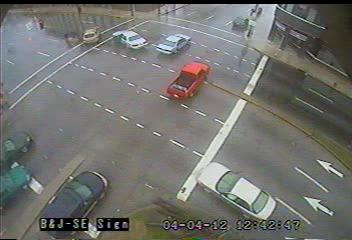
\includegraphics[width=5.55cm, height=3cm]{Imgs/Orig_0412041242.jpg}}
%  \vspace{2.0cm}
  \centerline{(a) Original Image}\medskip
\end{minipage}
%
\begin{minipage}[b]{0.3333\linewidth}
  \centering
  \centerline{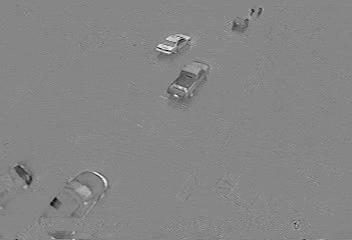
\includegraphics[width=5.55cm, height=3cm]{Imgs/SP_Intensity_0412041242}}
%  \vspace{1.5cm}
  \centerline{(b) Intensity Sparse Image}\medskip
\end{minipage}
\hfill
\begin{minipage}[b]{0.3333\linewidth}
  \centering
  \centerline{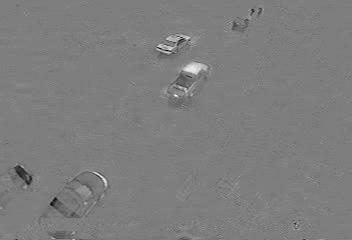
\includegraphics[width=5.55cm, height=3cm]{Imgs/SP_IMG_R_0412041242.jpg}}
%  \vspace{1.5cm}
  \centerline{(c) Red Channel Sparse Image}\medskip
\end{minipage}
%
\caption{Visual Comparison of Robust PCA on the Intensity Channel  and the Red Color Channel}
\label{fig:colorComp}
\medskip
%
\end{figure*}

\begin{figure*}[htb]

\begin{minipage}[b]{0.3333\linewidth}
  \centering
  \centerline{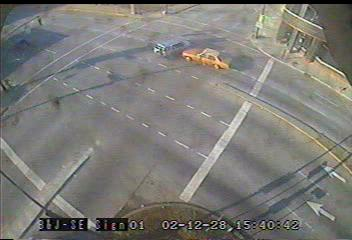
\includegraphics[width=5.55cm, height=3cm]{Imgs/Orig_1228021540.jpg}}
%  \vspace{2.0cm}
  \centerline{(a) Original Image}\medskip
\end{minipage}
%
\begin{minipage}[b]{0.3333\linewidth}
  \centering
  \centerline{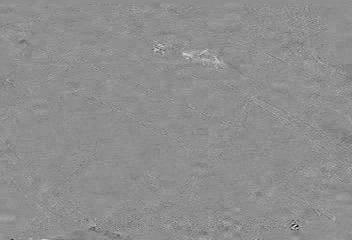
\includegraphics[width=5.55cm, height=3cm]{Imgs/SP_IMG_R_1228021540.jpg}}
%  \vspace{1.5cm}
  \centerline{(b) Robust PCA Sparse Image}\medskip
\end{minipage}
\hfill
\begin{minipage}[b]{0.3333\linewidth}
  \centering
  \centerline{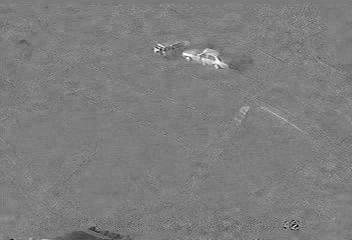
\includegraphics[width=5.55cm, height = 3cm]{Imgs/SP_IMG_Reduced_1228021540.jpg}}
%  \vspace{1.5cm}
  \centerline{(c) Reduced Robust PCA Sparse Image}\medskip
\end{minipage}
%
\caption{Reduced Frames Comparison}
\label{fig:reduceComp}
%
\end{figure*}


When given a data matrix M, the goal of Robust PCA is to decompose it into a low-rank matrix L and a sparse matrix S. To do this, each of the video frames is vectorized and stacked as a column in the matrix M. Upon closer inspection, one will notice that the columns are highly correlated. This is expected considering that the video was obtained using a stationary camera. Given that the background of a video lies on a low-dimensional subspace, we will see that the columns of L contain the background of each video frame and S contains the sparse deviations from that background, better known as foreground. Therefore, when doing background subtraction, one simply performs Robust PCA on the entire sequence and does further processing solely on the sparse error frames.


\subsection{Robust PCA on Individual Color Channels}

While many works acknowledge the merit of using Robust PCA for background subtraction, very few have introduced modifications to improve foreground detection. As such, we consider performing Robust PCA on all three of the color channels of a video sequence rather than just on the intensity channel. Now for each frame we have three sparse responses corresponding to each of the color channels. To ensure that an object detected with high confidence in one color channel is maintained in the final result, we take the maximum response across the three color channels.

Consider the images in figure \ref{fig:colorComp}. After Robust PCA is performed on the intensity channel of the video sequence, we see in figure \ref{fig:colorComp}b that several of the moving cars can be easily separated from the background just using their intensities. The red car, however, does not seem to stand out  from the background intensity. On the other hand, when considering the image in figure \ref{fig:colorComp}c, we see that doing Robust PCA on the red color channel makes the red car very distinguishable. Given that we also take the maximum response across all the color channels, this high response will remain intact when extracting a foreground mask.

\subsection{Reducing Number of Frames and Post-Processing}

Now that we have a protocol in place to better detect colored objects, we turn our attention to detecting objects that have stopped moving. Ordinarily when a object has been stationary for a long period of time, the background subtraction algorithm considers it  to be a part of the background. Similarly with  Robust PCA, when an object is stationary it is no longer considered a sparse corruption. Rather, it is considered a basis element of the low-rank subspace and enters the frame's background. In figure 2, the cars shown in figure \ref{fig:reduceComp}a have been stationary for some time, therefore they are no longer considered foreground and appear very faintly in the sparse component, show in figure \ref{fig:reduceComp}b.
 
In order to prevent this from happening, we reduce the number of frames used when computing Robust PCA by taking frames in intervals of 10 By reducing the number of frames in which the stationary object appears, we are making the object look like a sparse corruption and therefore less likely to enter the low-rank subspace modeling the background. The appearance of the two stationary cars in figure \ref{fig:reduceComp}c verifies our hypothesis. The reader may have noticed that by using a reduced number of frames in Robust PCA, the remaining frames will not have their own low-rank and sparse components. This is not a problem given that the scene was captured using a stationary camera. For each frame, we can simply take the nearest background image and subtract it to extract the sparse component.

After obtaining the sparse component of each video frame, we notice that they possess a fair amount of speckled noise. A classical approach to de-noising an image is through shrinking the wavelet coefficients via a hard or soft threshold \cite{Donoho95}. We apply a hard threshold to each sparse image to obtain a smoother response to be used during evaluation.


\begin{figure}[t]

\begin{minipage}[b]{0.48\linewidth}
  \centering
  \centerline{
\includegraphics[width=4cm, height=3cm]{Imgs/0112051333.png}}
%  \vspace{2.0cm}
  \centerline{(a) Ground Truth Labels}\medskip
\end{minipage}
%\hfill
\begin{minipage}[b]{0.48\linewidth}
  \centering
  \centerline{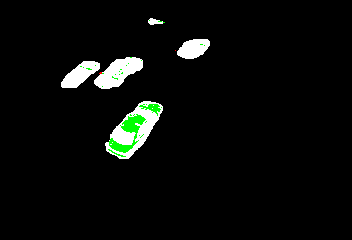
\includegraphics[width=4cm, height=3cm]{Imgs/0112051333_gmm_rwg.png}}
%  \vspace{1.5cm}
  \centerline{(b) GMM Result}\medskip
\end{minipage}

\begin{minipage}[b]{0.48\linewidth}
  \centering
  \centerline{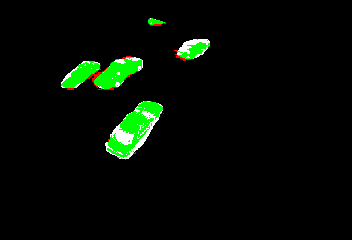
\includegraphics[width=4cm, height =3cm]{Imgs/0112051333_rpca_rwg.png}}
%  \vspace{1.5cm}
  \centerline{(c) RPCA Result}\medskip
\end{minipage}
%\hfill
\begin{minipage}[b]{0.48\linewidth}
  \centering
  \centerline{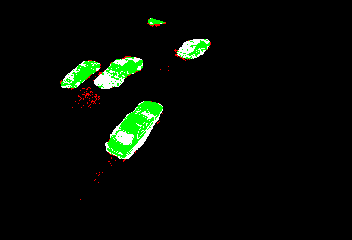
\includegraphics[width=4cm, height = 3cm]{Imgs/0112051333_grasta_rwg.png}}
%  \vspace{1.5cm}
  \centerline{(d) GRASTA Result}\medskip
\end{minipage}

\caption{Method Comparison I}
\label{fig:methodComp1}
%
\end{figure}


\begin{figure}[t]

\begin{minipage}[b]{0.48\linewidth}
  \centering
  \centerline{
\includegraphics[width=4cm, height=3cm]{Imgs/0412041242.png}}
%  \vspace{2.0cm}
  \centerline{(a) Ground Truth Labels}\medskip
\end{minipage}
%\hfill
\begin{minipage}[b]{0.48\linewidth}
  \centering
  \centerline{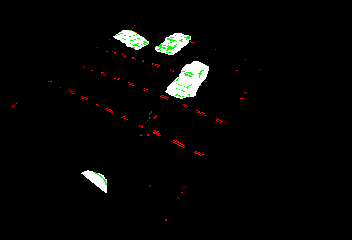
\includegraphics[width=4cm, height=3cm]{Imgs/0412041242_gmm_rwg.png}}
%  \vspace{1.5cm}
  \centerline{(b) GMM Result}\medskip
\end{minipage}

\begin{minipage}[b]{0.48\linewidth}
  \centering
  \centerline{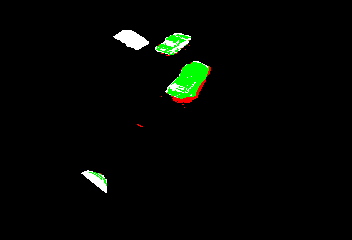
\includegraphics[width=4cm, height =3cm]{Imgs/0412041242_rpca_rwg.png}}
%  \vspace{1.5cm}
  \centerline{(c) RPCA Result}\medskip
\end{minipage}
%\hfill
\begin{minipage}[b]{0.48\linewidth}
  \centering
  \centerline{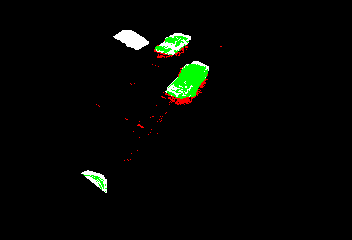
\includegraphics[width=4cm, height = 3cm]{Imgs/0412041242_grasta_rwg.png}}
%  \vspace{1.5cm}
  \centerline{(d) GRASTA Result}\medskip
\end{minipage}

\caption{Method Comparison II}
\label{fig:methodComp2}
%
\end{figure}









\section{Experimental Results}
%\label{sec:pagestyle}



(Cite Toyota Dataset?)

\section{Conclusions}
%\label{sec:typestyle}



% References should be produced using the bibtex program from suitable
% BiBTeX files (here: strings, refs, manuals). The IEEEbib.bst bibliography
% style file from IEEE produces unsorted bibliography list.
% -------------------------------------------------------------------------
\bibliographystyle{IEEEbib}
\bibliography{strings,refs}

\end{document}
